% answers.tex —— 1987 年·全国卷·理科 · 参考答案与详细解析片段
% 由 tools/generate_projects.py 依来源总账自 1987/1987_数学真题_全国理_试题.md + 1987/1987_数学真题_全国理_解析正文.md + 1987/1987_数学真题_全国理_答案要点.md 生成，勿手改（改源 MD 后重跑）


\begin{gktip}
固定源 PDF 只有一页原卷题面，原卷页码为 30，不含答案和解析页。下列推导均为本库独立复算。第 22 题照录了固定源中极限下标与表达式变量不一致的疑点；在疑点未裁决前，不把条件修订后的结果冒充为原题答案。
\end{gktip}

\begin{answer}
\gksolhead{1}{}

\textbf{题目}：

设 $S,T$ 是两个非空集合，且 $S\nsubseteq T,\ T\nsubseteq S$，令 $X=S\cap T$，那么 $S\cup X$ 等于\mbox{（　　）}

（A）$X$　　（B）$T$　　（C）$\varnothing$　　（D）$S$

\Needspace{4\baselineskip}
\textbf{解析}

\Needspace{5\baselineskip}
集合吸收律给出

\nopagebreak[4]
\[
S\cup X=S\cup(S\cap T)=S.
\]

所以答案为 D。

\gkanswer{答案：D}

\end{answer}
\begin{answer}
\gksolhead{2}{}

\textbf{题目}：

\Needspace{5\baselineskip}
设椭圆方程为

\nopagebreak[4]
\[
\frac{x^2}{a^2}+\frac{y^2}{b^2}=1\qquad(a>b>0),
\]

令 $c=\sqrt{a^2-b^2}$，那么它的准线方程为\mbox{（　　）}

（A）$y=\pm\dfrac{a^2}{c}$　　（B）$y=\pm\dfrac{b^2}{c}$

（C）$x=\pm\dfrac{a^2}{c}$　　（D）$x=\pm\dfrac{b^2}{c}$

\Needspace{4\baselineskip}
\textbf{解析}

\Needspace{5\baselineskip}
椭圆长轴在 $x$ 轴上，离心率为 $e=c/a$，准线为

\nopagebreak[4]
\[
x=\pm\frac ae=\pm\frac{a^2}{c}.
\]

所以答案为 C。

\gkanswer{答案：C}

\end{answer}
\begin{answer}
\gksolhead{3}{}

\textbf{题目}：

设 $a,b$ 是满足 $ab<0$ 的实数，那么\mbox{（　　）}

（A）$|a+b|>|a-b|$　　（B）$|a+b|<|a-b|$

（C）$|a-b|<\bigl||a|-|b|\bigr|$　　（D）$|a-b|<|a|+|b|$

\Needspace{4\baselineskip}
\textbf{解析}

\Needspace{5\baselineskip}
由 $ab<0$ 可知 $ab$ 为负数。比较平方：

\nopagebreak[4]
\[
(a+b)^2-(a-b)^2=4ab<0.
\]

因此 $|a+b|<|a-b|$，答案为 B。

\gkanswer{答案：B}

\end{answer}
\begin{answer}
\gksolhead{4}{}

\textbf{题目}：

已知 $E,F,G,H$ 为空间中的四个点，设命题甲：点 $E,F,G,H$ 不共面；命题乙：直线 $EF$ 和 $GH$ 不相交。那么\mbox{（　　）}

（A）甲是乙的充分条件，但不是必要条件

（B）甲是乙的必要条件，但不是充分条件

（C）甲是乙的充要条件

（D）甲不是乙的充分条件，也不是乙的必要条件

\Needspace{4\baselineskip}
\textbf{解析}

若 $E,F,G,H$ 不共面，而直线 $EF$ 与 $GH$ 相交，则相交的两条直线确定一个平面，四个点将共面，矛盾。因此甲是乙的充分条件。

但乙不是甲的必要条件：四点可以共面，且 $EF$ 与 $GH$ 为平行直线而不相交。因此甲不是乙的必要条件，答案为 A。

\gkanswer{答案：A}

\end{answer}
\begin{answer}
\gksolhead{5}{}

\textbf{题目}：

在区间 $(-\infty,0)$ 上为增函数的是\mbox{（　　）}

（A）$y=-\log_{\frac12}(-x)$　　（B）$y=\dfrac{x}{1-x}$

（C）$y=-(x+1)^2$　　（D）$y=1+x^2$

\Needspace{4\baselineskip}
\textbf{解析}

\Needspace{5\baselineskip}
选项（B）中

\nopagebreak[4]
\[
\left(\frac{x}{1-x}\right)'=\frac1{(1-x)^2}>0,
\]

所以它在 $(-\infty,0)$ 上递增，答案为 B。

\gkanswer{答案：B}

\end{answer}
\begin{answer}
\gksolhead{6}{}

\textbf{题目}：

\Needspace{5\baselineskip}
要得到函数

\nopagebreak[4]
\[
y=\sin\left(2x-\frac\pi3\right)
\]

的图象，只需将函数 $y=\sin2x$ 的图象（如图）\mbox{（　　）}
\nopagebreak[4]
\begin{center}% 1987 年全国卷理科第 6 题：y=sin 2x 图象
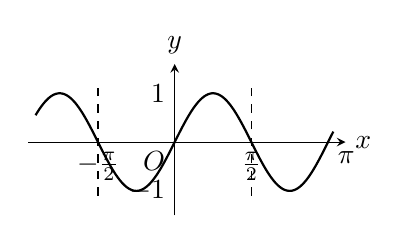
\begin{tikzpicture}[scale=0.62,>=stealth]
  \draw[->] (-3.0,0)--(3.5,0) node[right] {$x$};
  \draw[->] (0,-1.5)--(0,1.6) node[above] {$y$};
  \draw[thick,domain=-2.85:3.25,samples=160]
    plot (\x,{sin(114.592*\x)});
  \draw[dashed] (-1.57,-1.1)--(-1.57,1.1);
  \draw[dashed] (1.57,-1.1)--(1.57,1.1);
  \node[below] at (-1.57,0) {$-\frac\pi2$};
  \node[below] at (1.57,0) {$\frac\pi2$};
  \node[below right] at (3.14,0) {$\pi$};
  \node[left] at (0,1) {$1$};
  \node[left] at (0,-1) {$-1$};
  \node[below left] at (0,0) {$O$};
\end{tikzpicture}
\end{center}
\nopagebreak[4]
（A）向左平行移动 $\dfrac\pi3$　　（B）向右平行移动 $\dfrac\pi3$

（C）向左平行移动 $\dfrac\pi6$　　（D）向右平行移动 $\dfrac\pi6$

\Needspace{4\baselineskip}
\textbf{解析}

\nopagebreak[4]
\[
\sin\left(2x-\frac\pi3\right)
=\sin\left(2\left(x-\frac\pi6\right)\right).
\]

所以将 $y=\sin2x$ 的图象向右平移 $\dfrac\pi6$，答案为 D。

\gkanswer{答案：D}

\end{answer}
\begin{answer}
\gksolhead{7}{}

\textbf{题目}：

\Needspace{5\baselineskip}
极坐标方程

\nopagebreak[4]
\[
\rho=\sin\theta+2\cos\theta
\]

所表示的曲线是\mbox{（　　）}

（A）直线　　（B）圆　　（C）双曲线　　（D）抛物线

\Needspace{4\baselineskip}
\textbf{解析}

\Needspace{5\baselineskip}
由极坐标和直角坐标的关系

\nopagebreak[4]
\[
\rho^2=x^2+y^2,\qquad \rho\sin\theta=y,\qquad \rho\cos\theta=x,
\]

\Needspace{5\baselineskip}
得

\nopagebreak[4]
\[
x^2+y^2=y+2x.
\]

\Needspace{5\baselineskip}
即

\nopagebreak[4]
\[
(x-1)^2+\left(y-\frac12\right)^2=\frac54.
\]

这是一个圆，答案为 B。

\gkanswer{答案：B}

\end{answer}
\begin{answer}
\gksolhead{8}{}

\textbf{题目}：

\Needspace{5\baselineskip}
函数

\nopagebreak[4]
\[
y=\arccos(\cos x)\qquad x\in\left[-\frac\pi2,\frac\pi2\right]
\]

的图象是\mbox{（　　）}
\nopagebreak[4]
\begin{center}% 1987 年全国卷理科第 8 题：y=arccos(cos x) 在 [-pi/2,pi/2] 上的四个图象选项
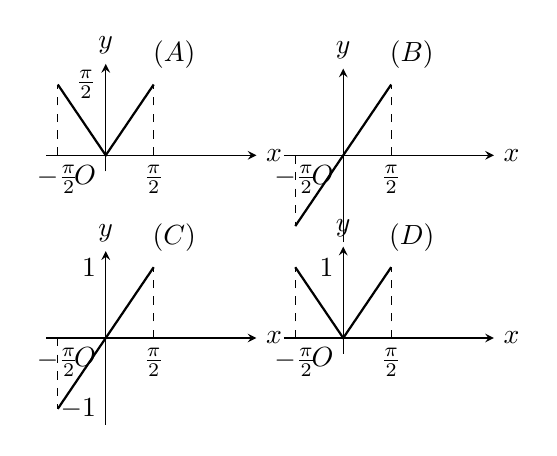
\begin{tikzpicture}[scale=0.58,>=stealth]
  \node at (1.5,2.2) {$(A)$};
  \draw[->] (-1.3,0)--(3.3,0) node[right] {$x$};
  \draw[->] (0,-0.35)--(0,2.0) node[above] {$y$};
  \draw[thick] (-1.05,1.55)--(0,0)--(1.05,1.55);
  \draw[dashed] (-1.05,0)--(-1.05,1.55) (1.05,0)--(1.05,1.55);
  \node[below] at (-1.05,0) {$-\frac\pi2$};
  \node[below] at (1.05,0) {$\frac\pi2$};
  \node[left] at (0,1.55) {$\frac\pi2$};
  \node[below left] at (0,0) {$O$};

  \begin{scope}[xshift=5.2cm]
    \node at (1.5,2.2) {$(B)$};
    \draw[->] (-1.3,0)--(3.3,0) node[right] {$x$};
    \draw[->] (0,-1.9)--(0,1.9) node[above] {$y$};
    \draw[thick] (-1.05,-1.55)--(1.05,1.55);
    \draw[dashed] (-1.05,0)--(-1.05,-1.55) (1.05,0)--(1.05,1.55);
    \node[below] at (-1.05,0) {$-\frac\pi2$};
    \node[below] at (1.05,0) {$\frac\pi2$};
    \node[below left] at (0,0) {$O$};
  \end{scope}

  \begin{scope}[yshift=-4.0cm]
    \node at (1.5,2.2) {$(C)$};
    \draw[->] (-1.3,0)--(3.3,0) node[right] {$x$};
    \draw[->] (0,-1.9)--(0,1.9) node[above] {$y$};
    \draw[thick] (-1.05,-1.55)--(1.05,1.55);
    \draw[dashed] (-1.05,0)--(-1.05,-1.55) (1.05,0)--(1.05,1.55);
    \node[below] at (-1.05,0) {$-\frac\pi2$};
    \node[below] at (1.05,0) {$\frac\pi2$};
    \node[left] at (0,1.55) {$1$};
    \node[left] at (0,-1.55) {$-1$};
    \node[below left] at (0,0) {$O$};
  \end{scope}

  \begin{scope}[xshift=5.2cm,yshift=-4.0cm]
    \node at (1.5,2.2) {$(D)$};
    \draw[->] (-1.3,0)--(3.3,0) node[right] {$x$};
    \draw[->] (0,-0.35)--(0,2.0) node[above] {$y$};
    \draw[thick] (-1.05,1.55)--(0,0)--(1.05,1.55);
    \draw[dashed] (-1.05,0)--(-1.05,1.55) (1.05,0)--(1.05,1.55);
    \node[below] at (-1.05,0) {$-\frac\pi2$};
    \node[below] at (1.05,0) {$\frac\pi2$};
    \node[left] at (0,1.55) {$1$};
    \node[below left] at (0,0) {$O$};
  \end{scope}
\end{tikzpicture}
\end{center}
\nopagebreak[4]
\Needspace{4\baselineskip}
\textbf{解析}

\Needspace{5\baselineskip}
在 $x\in[-\pi/2,\pi/2]$ 上，$\cos x$ 的值域为 $[0,1]$，并且

\nopagebreak[4]
\[
\arccos(\cos x)=|x|.
\]

因此图象是顶点在原点、两端点为 $\left(-\dfrac\pi2,\dfrac\pi2\right)$ 和 $\left(\dfrac\pi2,\dfrac\pi2\right)$ 的折线，答案为 A。

\gkanswer{答案：A}

\end{answer}
\begin{answer}
\gksolhead{9}{}

\textbf{题目}：

\Needspace{5\baselineskip}
求函数

\nopagebreak[4]
\[
y=\tan\frac{2x}{3}
\]

的周期。

\Needspace{4\baselineskip}
\textbf{解析}

\Needspace{5\baselineskip}
$\tan u$ 的最小正周期为 $\pi$。令 $u=2x/3$，于是

\nopagebreak[4]
\[
\frac23T=\pi,
\qquad
T=\frac{3\pi}{2}.
\]

\gkanswer{答案：$\dfrac{3\pi}{2}$}

\end{answer}
\begin{answer}
\gksolhead{10}{}

\textbf{题目}：

\Needspace{5\baselineskip}
已知方程

\nopagebreak[4]
\[
\frac{x^2}{2+\lambda}-\frac{y^2}{1+\lambda}=1
\]

表示双曲线，求 $\lambda$ 的范围。

\Needspace{4\baselineskip}
\textbf{解析}

\Needspace{5\baselineskip}
要表示双曲线，两个分母须同号且都不为零：

\nopagebreak[4]
\[
(\lambda+2)(\lambda+1)>0.
\]

\Needspace{5\baselineskip}
故

\nopagebreak[4]
\[
\lambda\in(-\infty,-2)\cup(-1,+\infty).
\]

\gkanswer{答案：$\lambda<-2$ 或 $\lambda>-1$}

\end{answer}
\begin{answer}
\gksolhead{11}{}

\textbf{题目}：

若 $(1+x)^n$ 的展开式中，$x^3$ 的系数等于 $x$ 的系数的 7 倍，求 $n$。

\Needspace{4\baselineskip}
\textbf{解析}

\Needspace{5\baselineskip}
由二项式系数

\nopagebreak[4]
\[
\binom n3=7\binom n1=7n,
\]

\Needspace{5\baselineskip}
得

\nopagebreak[4]
\[
(n-1)(n-2)=42.
\]

取正整数解 $n=8$。

\gkanswer{答案：$8$}

\end{answer}
\begin{answer}
\gksolhead{12}{}

\textbf{题目}：

\Needspace{5\baselineskip}
求极限

\nopagebreak[4]
\[
\lim_{n\to\infty}\left(
\frac1{n^2+1}+\frac2{n^2+1}+\frac3{n^2+1}
+\cdots+\frac{2n}{n^2+1}
\right).
\]

\Needspace{4\baselineskip}
\textbf{解析}

\nopagebreak[4]
\[
\lim_{n\to\infty}
\frac{1+2+\cdots+2n}{n^2+1}
=\lim_{n\to\infty}\frac{n(2n+1)}{n^2+1}=2.
\]

\gkanswer{答案：$2$}

\end{answer}
\begin{answer}
\gksolhead{13}{}

\textbf{题目}：

在抛物线 $y=4x^2$ 上求一点，使该点到直线 $y=4x-5$ 的距离为最短。

\Needspace{4\baselineskip}
\textbf{解析}

\Needspace{5\baselineskip}
设抛物线上的点为 $(x,4x^2)$。它到直线 $4x-y-5=0$ 的距离为

\nopagebreak[4]
\[
d(x)=\frac{|4x^2-4x+5|}{\sqrt{17}}.
\]

\Needspace{5\baselineskip}
因为

\nopagebreak[4]
\[
4x^2-4x+5=4\left(x-\frac12\right)^2+4>0,
\]

\Needspace{5\baselineskip}
只需令 $x=1/2$，得到点

\nopagebreak[4]
\[
\left(\frac12,1\right).
\]

\gkanswer{答案：$\left(\dfrac12,1\right)$}

\end{answer}
\begin{answer}
\gksolhead{14}{}

\textbf{题目}：

由数字 $1,2,3,4,5$ 组成没有重复数字且数字 1 与 2 不相邻的五位数。求这种五位数的个数。

\Needspace{4\baselineskip}
\textbf{解析}

五个数字全排列有 $5!=120$ 种。1、2 相邻时作为一个整体，内部有 2 种顺序，与其他三个数字共作 $4!$ 排列，故有 $2\cdot4!=48$ 种。

\Needspace{5\baselineskip}
所求个数为

\nopagebreak[4]
\[
5!-2\cdot4!=72.
\]

\gkanswer{答案：$72$}

\end{answer}
\begin{answer}
\gksolhead{15}{}

\textbf{题目}：

一个正三棱台的下底和上底的周长分别为 $30\text{ cm}$ 和 $12\text{ cm}$，而侧面积等于两底面积之差，求斜高。

\Needspace{4\baselineskip}
\textbf{解析}

\Needspace{5\baselineskip}
设正三棱台两底边长分别为 $10$ 和 $4$，斜高为 $l$。则侧面积为

\nopagebreak[4]
\[
\frac{30+12}{2}l=21l.
\]

\Needspace{5\baselineskip}
两底面积之差为

\nopagebreak[4]
\[
\frac{\sqrt3}{4}(10^2-4^2)=21\sqrt3.
\]

\Needspace{5\baselineskip}
由题设 $21l=21\sqrt3$，故

\nopagebreak[4]
\[
l=\sqrt3\text{ cm}.
\]

\gkanswer{答案：$3\pi$}

\end{answer}
\begin{answer}
\gksolhead{16}{}

\textbf{题目}：

\Needspace{5\baselineskip}
求

\nopagebreak[4]
\[
\sin10^\circ\sin30^\circ\sin50^\circ\sin70^\circ
\]

的值。

\Needspace{4\baselineskip}
\textbf{解析}

\Needspace{5\baselineskip}
利用积化和差：

\nopagebreak[4]
\[
\sin10^\circ\sin50^\circ
=\frac{\cos40^\circ-\cos60^\circ}{2}.
\]

\Needspace{5\baselineskip}
又

\nopagebreak[4]
\[
\sin10^\circ\sin50^\circ\sin70^\circ=\frac18,
\]

\Needspace{5\baselineskip}
所以

\nopagebreak[4]
\[
\sin10^\circ\sin30^\circ\sin50^\circ\sin70^\circ
=\frac1{16}.
\]

\gkanswer{答案：$\dfrac1{16}$}

\end{answer}
\begin{answer}
\gksolhead{17}{}

\textbf{题目}：

\Needspace{5\baselineskip}
如图，三棱锥 $P-ABC$ 中，已知 $PA\perp BC,\ PA=BC=L$，$PA,BC$ 的公垂线 $ED=h$。求证：三棱锥 $P-ABC$ 的体积

\nopagebreak[4]
\[
V=\frac16L^2h.
\]
\nopagebreak[4]
\begin{center}% 1987 年全国卷理科第 17 题：三棱锥及公垂线
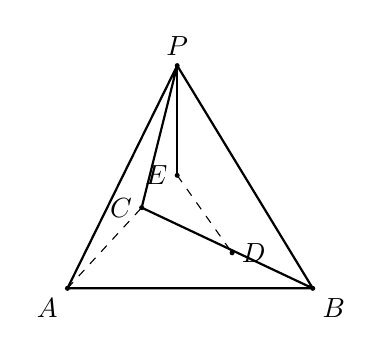
\begin{tikzpicture}[scale=0.82,>=stealth]
  \coordinate (P) at (1.7,3.45);
  \coordinate (A) at (0,0);
  \coordinate (B) at (3.8,0);
  \coordinate (C) at (1.15,1.25);
  \coordinate (E) at (1.7,1.75);
  \coordinate (D) at (2.55,0.55);
  \draw[thick] (P)--(A) (P)--(B) (P)--(C) (A)--(B) (B)--(C);
  \draw[dashed] (A)--(C) (E)--(D);
  \draw[thick] (E)--(P);
  \fill (P) circle (1.1pt) node[above] {$P$};
  \fill (A) circle (1.1pt) node[below left] {$A$};
  \fill (B) circle (1.1pt) node[below right] {$B$};
  \fill (C) circle (1.1pt) node[left] {$C$};
  \fill (E) circle (1.1pt) node[left] {$E$};
  \fill (D) circle (1.1pt) node[right] {$D$};
\end{tikzpicture}
\end{center}
\nopagebreak[4]
\Needspace{4\baselineskip}
\textbf{解析}

取 $PA,BC,ED$ 为三个互相垂直的方向。四面体体积的六倍等于对应三个方向向量的混合积绝对值。

\Needspace{5\baselineskip}
由 $PA=BC=L$ 且 $PA\perp BC$，这两个方向给出面积因子 $L^2$；两条异面直线的公垂线长为 $ED=h$，因此

\nopagebreak[4]
\[
6V=L^2h.
\]

\Needspace{5\baselineskip}
于是

\nopagebreak[4]
\[
V=\frac16L^2h.
\]

\gkanswer{答案：$V=\dfrac16L^2h$}

\end{answer}
\begin{answer}
\gksolhead{18}{}

\textbf{题目}：

\Needspace{5\baselineskip}
设对所有实数 $x$，不等式

\nopagebreak[4]
\[
x^2\log_2\frac{4(a+1)}a
+2x\log_2\frac{2a}{a+1}
+\log_2\frac{(a+1)^2}{4a^2}>0
\]

恒成立，求 $a$ 的取值范围。

\Needspace{4\baselineskip}
\textbf{解析}

\Needspace{5\baselineskip}
令

\nopagebreak[4]
\[
q=\log_2\frac{2a}{a+1}.
\]

\Needspace{5\baselineskip}
则

\nopagebreak[4]
\[
\log_2\frac{4(a+1)}a=3-q,\qquad
\log_2\frac{(a+1)^2}{4a^2}=-2q.
\]

\Needspace{5\baselineskip}
原式成为

\nopagebreak[4]
\[
(3-q)x^2+2qx-2q>0.
\]

\Needspace{5\baselineskip}
对所有实数 $x$ 恒正，先由 $x=0$ 得 $q<0$。此时二次项系数为正，判别式为

\nopagebreak[4]
\[
\Delta=4q^2-4(3-q)(-2q)=4q(6-q)<0.
\]

\Needspace{5\baselineskip}
因此条件等价于

\nopagebreak[4]
\[
0<\frac{2a}{a+1}<1.
\]

\Needspace{5\baselineskip}
结合对数真数的定义域，得到

\nopagebreak[4]
\[
0<a<1.
\]

\gkanswer{答案：$0<a<1$}

\end{answer}
\begin{answer}
\gksolhead{19}{}

\textbf{题目}：

\Needspace{5\baselineskip}
设复数 $z_1$ 和 $z_2$ 满足关系式

\nopagebreak[4]
\[
z_1\overline{z_2}+\overline A z_1+A\overline{z_2}=0,
\]

其中 $A$ 为不等于 0 的复数。证明：

\Needspace{5\baselineskip}
（1） 证明：

\nopagebreak[4]
\[
|z_1+A||z_2+A|=|A|^2
\]
；

\Needspace{5\baselineskip}
（2） 证明：

\nopagebreak[4]
\[
\frac{z_1+A}{z_2+A}
=\left|
\frac{\overline{z_1}+\overline A}
{\overline{z_2}+\overline A}
\right|
\]
。

\Needspace{4\baselineskip}
\textbf{解析}

\gksubpart{（1）}

\Needspace{5\baselineskip}
由题设加上 $|A|^2=A\overline A$：

\nopagebreak[4]
\[
(z_1+A)(\overline{z_2}+\overline A)=|A|^2.
\]

\Needspace{5\baselineskip}
取绝对值得

\nopagebreak[4]
\[
|z_1+A||z_2+A|=|A|^2.
\]

\gksubpart{（2）}

\Needspace{5\baselineskip}
再除以 $|z_2+A|^2$，得到

\nopagebreak[4]
\[
\frac{z_1+A}{z_2+A}
=\frac{|A|^2}{|z_2+A|^2}
=\left|
\frac{\overline{z_1}+\overline A}
{\overline{z_2}+\overline A}
\right|.
\]

\gkanswer{答案（1）：$|z_1+A||z_2+A|=|A|^2$}

\gkanswer{答案（2）：$\displaystyle\frac{z_1+A}{z_2+A}=\left|\frac{\overline{z_1}+\overline A}{\overline{z_2}+\overline A}\right|$}

\end{answer}
\begin{answer}
\gksolhead{20}{}

\textbf{题目}：

\Needspace{5\baselineskip}
设数列 $a_1,a_2,\ldots,a_n,\ldots$ 的前 $n$ 项的和 $S_n$ 与 $a_n$ 的关系是

\nopagebreak[4]
\[
S_n=-ba_n+1-\frac{1}{(1+b)^n},
\]

其中 $b$ 是与 $n$ 无关的常数，且 $b\ne-1$。

（1） 求 $a_n$ 和 $a_{n-1}$ 的关系式；

（2） 写出用 $n$ 和 $b$ 表示 $a_n$ 的表达式；

\Needspace{5\baselineskip}
（3） 当 $0<b<1$ 时，求极限

\nopagebreak[4]
\[
\lim_{n\to\infty}S_n.
\]

\Needspace{4\baselineskip}
\textbf{解析}

\gksubpart{（1）}

\Needspace{5\baselineskip}
由 $S_n-S_{n-1}=a_n$，对 $n\ge2$ 有

\nopagebreak[4]
\[
(1+b)a_n=ba_{n-1}+\frac{b}{(1+b)^n}.
\]

\Needspace{5\baselineskip}
当 $n=1$ 时，$S_1=a_1$ 给出

\nopagebreak[4]
\[
a_1=\frac{b}{(1+b)^2}.
\]

\gksubpart{（2）}

\Needspace{5\baselineskip}
递推求和可得

\nopagebreak[4]
\[
a_n=\frac{b(1+b+\cdots+b^{n-1})}{(1+b)^{n+1}}.
\]

\gksubpart{（3）}

\Needspace{5\baselineskip}
当 $0<b<1$ 时，分子中的等比和有界，而分母趋于无穷，所以 $a_n\to0$。由题设

\nopagebreak[4]
\[
S_n=-ba_n+1-\frac{1}{(1+b)^n},
\]

\Needspace{5\baselineskip}
得到

\nopagebreak[4]
\[
\lim_{n\to\infty}S_n=1.
\]

\gkanswer{答案（1）：$\displaystyle (1+b)a_n=ba_{n-1}+\frac{b}{(1+b)^n}$}

\gkanswer{答案（2）：$\displaystyle a_n=\frac{b(1+b+\cdots+b^{n-1})}{(1+b)^{n+1}}$}

\gkanswer{答案（3）：$\displaystyle\lim_{n\to\infty}S_n=1\quad(0<b<1)$}

\end{answer}
\begin{answer}
\gksolhead{21}{}

\textbf{题目}：

\Needspace{5\baselineskip}
定长为 $3$ 的线段 $AB$ 的两端点在抛物线

\nopagebreak[4]
\[
y^2=x
\]

上移动，记线段 $AB$ 的中点为 $M$，求点 $M$ 到 $y$ 轴的最短距离，并求此时点 $M$ 的坐标。

\Needspace{4\baselineskip}
\textbf{解析}

\Needspace{5\baselineskip}
设抛物线上的两个端点为

\nopagebreak[4]
\[
A=(u^2,u),\qquad B=(v^2,v).
\]

\Needspace{5\baselineskip}
令 $s=u+v,\ d=u-v$。由 $AB=3$ 得

\nopagebreak[4]
\[
(u^2-v^2)^2+(u-v)^2
=d^2(s^2+1)=9.
\]

\Needspace{5\baselineskip}
中点 $M$ 的横坐标为

\nopagebreak[4]
\[
x_M=\frac{u^2+v^2}{2}
=\frac{s^2+d^2}{4}
=\frac14\left(s^2+\frac9{s^2+1}\right).
\]

\Needspace{5\baselineskip}
令 $t=s^2\ge0$，需要最小化

\nopagebreak[4]
\[
t+\frac9{t+1}.
\]

\Needspace{5\baselineskip}
由导数

\nopagebreak[4]
\[
1-\frac9{(t+1)^2}=0
\]

\Needspace{5\baselineskip}
得 $t=2$，且此处取得最小值 $5$。所以

\nopagebreak[4]
\[
x_M^{\min}=\frac54.
\]

\Needspace{5\baselineskip}
当 $s=\pm\sqrt2$ 时，$y_M=s/2=\pm\sqrt2/2$。因此最短距离为 $\dfrac54$，对应点为

\nopagebreak[4]
\[
M=\left(\frac54,\frac{\sqrt2}{2}\right)
\]

\Needspace{5\baselineskip}
或

\nopagebreak[4]
\[
M=\left(\frac54,-\frac{\sqrt2}{2}\right).
\]

\gkanswer{答案：到 $y$ 轴的最短距离为 $\dfrac54$；此时 $M$ 为 $\left(\dfrac54,\dfrac{\sqrt2}{2}\right)$ 或 $\left(\dfrac54,-\dfrac{\sqrt2}{2}\right)$。}

\end{answer}
\begin{answer}
\gksolhead{22}{}

\textbf{题目}：

\Needspace{5\baselineskip}
求极限

\nopagebreak[4]
\[
\lim_{n\to\infty}\left(1-\frac1{2x}\right)^x.
\]

\begin{gktip}
\textbf{转录疑点}：原卷此处极限下标写 $n\to\infty$，但括号中的变量和指数写作 $x$；本题按固定源字面照录，未擅自把 $x$ 改成 $n$。
\end{gktip}

\Needspace{4\baselineskip}
\textbf{解析}

\Needspace{5\baselineskip}
固定源题面把极限变量写为 $n$，但被取极限的式子使用了 $x$：

\nopagebreak[4]
\[
\lim_{n\to\infty}\left(1-\frac1{2x}\right)^x.
\]

\Needspace{5\baselineskip}
按字面，$x$ 未随 $n$ 变化，因而不能从该式得到唯一的极限值。若独立确认原题应为

\nopagebreak[4]
\[
\lim_{n\to\infty}\left(1-\frac1{2n}\right)^n,
\]

则由标准极限得到 $e^{-1/2}$；这只是条件性结果，不能替代当前固定源题面。

\gkanswer{答案：固定源下标为 $n\to\infty$，但式中底数和指数为 $x$，按字面无法得到唯一的关于 $n$ 的极限；若按通常意图统一改为 $\displaystyle\lim_{n\to\infty}\left(1-\frac1{2n}\right)^n$，则值为 $e^{-1/2}$。}

\end{answer}
\begin{answer}
\gksolhead{23}{}

\textbf{题目}：

\Needspace{5\baselineskip}
设

\nopagebreak[4]
\[
y=x\ln(1+x^2),
\]

求 $y'$。

\Needspace{4\baselineskip}
\textbf{解析}

\Needspace{5\baselineskip}
直接使用乘积法则：

\nopagebreak[4]
\[
y'=\ln(1+x^2)+x\cdot\frac{2x}{1+x^2}
=\ln(1+x^2)+\frac{2x^2}{1+x^2}.
\]

\gkanswer{答案：$\displaystyle y'=\ln(1+x^2)+\frac{2x^2}{1+x^2}$}

\end{answer}